\begin{frame}{Bonnes pratiques dans le numérique}{Conseils 72-74/115}
\begin{block}{Afficher des pages d'erreur statiques}
Les pages d'erreurs (40x, 50x) doivent être les plus légères possibles, et même idéalement inexistantes. 
\end{block}
\begin{block}{Utiliser un serveur asynchrone}

La plupart des serveurs web augmentent leur consommation de mémoire vive au fur et à mesure des sollicitations. Les serveurs asynchrones demeurent très stables.

Les serveurs ( Nginx, node.js ou Gwan) utilisent le minimum de ressources. 
\end{block}

\begin{block}{Utiliser un CDN (Content Delivery Network)}
Certains fichiers (bibliothèques JavaScript, les feuilles de style CSS, les images) sont gourmands en ressources réseau, car ils sont généralement nombreux et de petite taille. Utiliser les CDN, rapprochent physiquement ces fichiers des internautes, générant de ce fait un gain important de bande passante et un meilleur temps de réponse.
\end{block}


\end{frame}


\begin{frame}{Bonnes pratiques dans le numérique}{Conseils 75-76/115}
\begin{block}{Utiliser un cache HTTP}
Les reverse proxies (Varnish, Squid ou Nginx) sont optimisés pour servir du contenu (pages HTML, images, etc.) en consommant le moins de cycles CPU. 
\end{block}
\begin{block}{Ajouter des entêtes Expires ou Cache-Control}
Les en-têtes définissent la durée de conservation d'une ressource dans le cache.
\begin{figure}
    \centering
    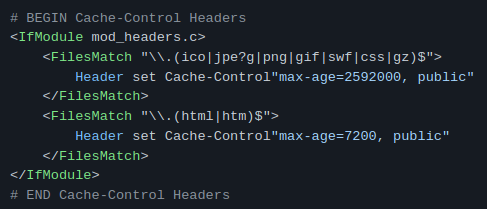
\includegraphics[scale=0.5]{chapitre2/wdd7/fig/c1.png}
\end{figure}
\end{block}
\end{frame}




\begin{frame}{Bonnes pratiques dans le numérique}{Conseils 76-78/115}
\begin{block}{Mettre en cache les réponses Ajax}
Les réponses Ajax qui seront inchangées dans un futur proche ne doivent pas être redemandées au serveur. Par conséquent, les mettre en cache économise la bande passante.
\end{block}

\begin{block}{Réduire au nécessaire les logs des serveurs}
Les logs des serveurs (web, applicatif, base de données) pouvant devenir très volumineux, il est recommandé de les configurer dans leur ensemble.
\begin{figure}
    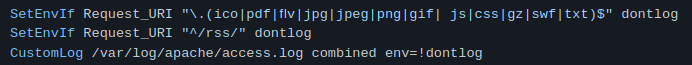
\includegraphics[scale=0.4]{chapitre2/wdd7/fig/c2.png}
\end{figure}
\end{block}

\begin{block}{Désactiver le DNS lookup d’Apache}
Quand un serveur web reçoit une requête HTTP, il enregistre cette information dans un log, en traduisant l’adresse IP de l’internaute en nom de domaine. 
\end{block}

\end{frame}


\begin{frame}{Bonnes pratiques dans le numérique}{Conseils 79-82/115}
\begin{block}{Apache Vhost : désactiver le AllowOverride}
 Le serveur HTTP Apache remonter toute la hiérarchie des répertoires pour y trouver un fichier .htaccess contenant des règles de surcharge. 
\end{block}
\begin{block}{Désactiver les logs binaires}
 Les logs binaires du serveur MySQL ou MariaDB peuvent être volumineux.
\end{block}

\begin{minipage}[b]{0.5\linewidth}
\begin{figure}
    
\includegraphics[scale=0.4]{chapitre2/wdd7/fig/c4.png}
    \centering
\end{figure}
\end{minipage}\hfill
\begin{minipage}[b]{0.5\linewidth}
\begin{figure}
    
\includegraphics[scale=0.4]{chapitre2/wdd7/fig/c3.png}
    \centering
\end{figure}
\end{minipage}\hfill


\begin{block}{Compresser les documents}
Un document pèse moins une fois compressé.
\end{block}

\begin{block}{Optimiser les PDF}
PDF adapté (taux d’échantillonnage et de compression des images, polices incorporées, résolution).
\end{block}

\end{frame}


\begin{frame}{Bonnes pratiques dans le numérique}{Conseils 83-85/115}
\begin{block}{Limiter les e-mails lourds et redondants}
Raisonner l'envoi d'e-mail automatiques (newsletters, gestion client, suivi de commande) en limitant leur nombre, les pièces jointes et le nombre de destinataires.
\end{block}

\begin{block}{Adapter les sons aux contextes d'écoute}
Privilégier 3 formats couvrant les 3 grandes plates-formes (Windows, Mac OS X et Linux) :
\begin{itemize}
    \item MP3 (MPEG-1 Audio Layer 3) ;
    \item  AAC (Advanced Audio Coding) ;
    \item Vorbis.
\end{itemize}
\end{block}

\begin{block}{Adapter les textes au web}
Ecrire des textes courts à l’aide d’un style direct.
\end{block}

\end{frame}

\begin{frame}{Bonnes pratiques dans le numérique}{Conseils 86-88/115}
\begin{block}{Adapter les vidéos aux contextes de visualisation}
Prévoir plusieurs formats (taille, frame rate, compression audio, etc.) selon le contexte de lecture des vidéos (ordinateur de bureau, tablette Wi-Fi, smartphone EDGE. ).
\end{block}

\begin{block}{N'utiliser que des fichiers double opt-in}
Le double opt-in est une pratique marketing consistant à demander le consentement du prospect, généralement par accord électronique en cochant une case, puis à faire valider ce consentement par l’envoi d’un e-mail de confirmation à l’adresse indiquée. 
\end{block}

\begin{block}{Limiter les outils d'analytics et les données collectées}
Les outils utilisés pour suivre les actions des utilisateurs utilisent souvent beaucoup de ressources coté client : requêtes nombreuses, fichiers javascripts supplémentaires chargés, utilisation de plusieurs domaines additionnels, envoi de cookie, ...
\end{block}

\end{frame}



\begin{frame}{Pause débunkage }{Parlons applications et dopamine}
\begin{figure}
    \centering
    
\includegraphics[scale=0.5]{chapitre2/wdd7/fig/dopa.png}
\end{figure}
\end{frame}

